\chapter{CONVECTION CORRELATION DEVELOPMENT AND VALIDATION}
\label{ch:Correlation}

\section{Correlation Optimization Methodology}
\label{sec:Correlation:Development:NelderMead}
	
To determine the convection correlations developed in this section, a correlation form was proposed, and the correlation parameters were determined through parameter estimation by using the \cite{NelderMead1965} simplex algorithm which is a direct search method used for finding the optimum value of the objective function. In our case, the objective function was the sum of the squared error of the outside Nusselt number. This method, however, is not fool proof and reasonable initial guesses and step sizes must be selected so that the solution converges on a global minimum, rather than a local minimum. Once a solution has been determined, the algorithm should then again be restarted using the optimized solution from the first iteration as the initial guess for the second iteration. This helps assure that the method has converged on the global solution.	
	
%A simplex algorithm developed by \cite{NelderMead1965} was used to optimize the outside Nusselt number convection correlations. The simplex method utilizes a heuristic method that either ``expands," ``contracts," or ``reflects" an optimization parameter, then checks to determine if the solution is `better' or `worse' than it was before the change. If the solution is better, the algorithm continues to move the parameter in that direction; if it is worse, it moves the parameter in the opposite direction. By this means, the simplex method searches to find the optimized solution.

In order to optimize the convection correlations developed in this chapter, the sum of the squared error for the outside Nusselt number was used as the optimization parameter to be minimized. To perform the optimization, the outside Nusselt number was defined primarily as a function of the modified Raleigh number. Other parameters such as the ratio of horizontal and vertical tube-tube spacing to outside pipe diameter ($\Delta x / D_o$ $\Delta y / D_o$) were also used to correlate SWHE performance. An example form of the correlation equation can be seen in Equation \ref{eq:Intro:LitRev:ClosedLoop:Hansen}, which is the correlation form use by \cite{Hansen2011}.

%\begin{equation}
%	\mbox{Nu}_{D,o,corr} = f(\mbox{Ra}_{D,o,exp}^*, \, a, \, b, \, \cdots)
%	\label{eq:Correlation:Development:NelderMead:NuCorr}
%\end{equation}

To perform the optimization, the squared error was determined from Equation \ref{eq:Correlation:Development:NelderMead:SQE}, which is the squared difference between the correlated Nusselt number and the experimental Nusselt number. Equation \ref{eq:Correlation:Development:NelderMead:SSQE} can then be used to determine the sum of the squared error which was then minimized using the simplex method.

\begin{equation}
	\mbox{SQE} = (\mbox{Nu}_{D,o,corr} - \mbox{Nu}_{D,o,exp})^2
	\label{eq:Correlation:Development:NelderMead:SQE}
\end{equation}

\begin{equation}
	\mbox{SSQE} = \sum_{n=1}^{N_{tot}} \mbox{SQE}
	\label{eq:Correlation:Development:NelderMead:SSQE}
\end{equation}


\section{Convection Correlations}
\label{sec:Correlation:IndivCorr}

\subsection{Convection Correlation Development Methodology}
\label{subsec:Correlation:Method}
	
Correlation development and optimization began initially by optimizing separate outside convection correlations based solely on statistical measures for each data set. This means that there was a specific external convection correlation for each of the pond and pool heat extraction and heat rejection data sets which were optimized to find the minimum sum of the squared error value as shown in Section \ref{sec:Correlation:Development:NelderMead}. However, once this was completed, it was observed in several heat transfer texts (\cite{IncroperaDewittBergmanLavine2007}, \cite{CengelGhajar2011}) that it is common for the Rayleigh number exponent to be set equal to 1/3 for free convection correlations.

It was also desirable, if feasible, that there be a simple scalar multiplier to switch from a correlation applicable in bodies of deep surface water where convective currents are likely to move freely, and bodies of surface water were convective currents are likely to be constrained. This is due to the discrepancy in Nusselt numbers observed between the pool and the pond data which was described in Section \ref{sec:ExpResult:FinalData}.

In an effort to test how well these qualifications could be met, a base data set was selected for heat extraction and heat rejection. Because the pond heat rejection data contained 27 SWHE geometrical variations, it was selected as the base heat rejection data set. This is in comparison to the alternative data set for the pool heat rejection data which only contained three separate SWHE geometrical configurations. For the base heat extraction data set, the pool data were selected. The pool heat extraction data set contained three SWHE geometrical variations, whereas the pond heat extraction data set contained only one, and thus, constituted the alternative data set.

Each base data set was then taken; Rayleigh number exponents were fixed at 1/3; and the external convection correlation was optimized to best fit the data. Then, the convection correlation derived from the base case was taken and a multiplier was then optimized to proportionally scale the correlation up or down to best fit the alternative data set.

Upon examining the results and comparing the results with the results from the individually optimized convection correlations, it was determined that this approach was acceptable. This was because Nusselt number RMSE increased by 3.7\% at most across all four data sets when compared to the individually optimized correlations. The average Nusselt number RMSE increase across the four data sets was 1.5\%. For the heat transfer comparisons, heat transfer RMSE increased by 5.9\% at most with an average increase of 2.4\%. From this, it was decided that the increase in error when compared to the experimental data was acceptable due to the simplifications the method offered.

In the following sections, the convection correlations developed for each data set will be outlined and shown. The Nusselt number validation and heat transfer validation against the experimental data will also be shown.


\subsection{Pond Heat Rejection Data Convection Correlation}
\label{subsec:Correlation:PondHeatRej}
		
		From the pond heat rejection data the convection correlation initially given by \cite{Hansen2011} in Equation \ref{eq:Intro:LitRev:ClosedLoop:Hansen} was updated based on the augmented data set with the additional eight heat SWHE configurations. Based on the testing, it was observed that a lower limit for Nusselt number existed which was not indicated in Equation \ref{eq:Intro:LitRev:ClosedLoop:Hansen}. This is visible in Figure \ref{fig:ExpResult:HeatRej:HansenData:AllPondHeatRejData} where 5 is approximately the lowest Nusselt number recorded.	To account for this lower limit, the form of the Nusselt number correlation was modified slightly to include a constant, as can be seen in Equation \ref{eq:Correlation:PondHeatRej:CorrForm}. Also included in the correlation is the scalar `$a$' which will be used later to scale the correlation to best fit the alternative data set. Applying the optimization algorithm yielded Equation \ref{eq:Correlation:PondHeatRej:Corr} as the final outside Nusselt number correlation for the pond heat rejection data set. The correlation's range of applicability can be seen Table \ref{tab:Correlation:PondHeatRej:RangeOfApp}.
		
\begin{equation}
	\mbox{Nu}_{D,o} = a \cdot \left( b+ c \cdot \mbox{Ra}_{D,o}^{* \, d} \cdot \left(\frac{\Delta y}{D_o}\right)^{e} \cdot \left(\frac{\Delta x}{D_o}\right)^{f} \right)
	\label{eq:Correlation:PondHeatRej:CorrForm}
\end{equation}

\begin{equation}
	\mbox{Nu}_{D,o} = 5+ 0.0317 \cdot \mbox{Ra}_{D,o}^{* \, 0.333} \cdot \left(\frac{\Delta y}{D_o}\right)^{0.344} \cdot \left(\frac{\Delta x}{D_o}\right)^{0.301}
	\label{eq:Correlation:PondHeatRej:Corr}
\end{equation}

	\begin{table}[h]
		\centering
		\caption[Range of applicability for pond heat rejection correlation]{Range of applicability for each parameter in Equation \ref{eq:Correlation:PondHeatRej:Corr}}
		\label{tab:Correlation:PondHeatRej:RangeOfApp}
		\begin{tabular}{r c c c l}
		0 & $\le$ &  $Ra_{D,o}^*$ & $\le$  & $6.0\cdot10^7$ \\
		1.3 in.\ (33 mm) & $\le$ & $\Delta y$ & $\le$ & 4.125 in.\ (105 mm) \\
		1.3 in.\ (33 mm) & $\le$ & $\Delta x$ & $\le$ & 4.125 in.\ (105 mm) \\
		1.05 in.\ (27 mm) & $\le$ &  $D_o$ &  $\le$ & 1.66 in.\ (42 mm) \\
		0.85 in.\ (22 mm) & $\le$ &  $D_i$ &  $\le$ & 1.36 in.\ (36 mm) \\
		\multicolumn{5}{c}{L = 500 ft.\ (153 m)} \\
		\end{tabular}
	\end{table}
			
			
\subsubsection{Experimental vs.\ Correlated Nusselt Number Comparison}

In order to validate Equation \ref{eq:Correlation:PondHeatRej:Corr}, the correlation was applied to the experimental data to check for consistency between the correlated results and the experimental data. This was done by taking the experimental modified Rayleigh number and SWHE geometrical configuration and applying Equation \ref{eq:Correlation:PondHeatRej:Corr} for each data point. The correlated and experimental Nusselt numbers can be seen in Figure \ref{fig:Correlation:PondHeatRej:NuComparison}. Also indicated in Figure \ref{fig:Correlation:PondHeatRej:NuComparison}, are the $\pm 25 \%$ $\pm 50 \%$ error bars, along with the unity line where correlated results vs.\ experimental data are equal.

\begin{figure}
	\centering
	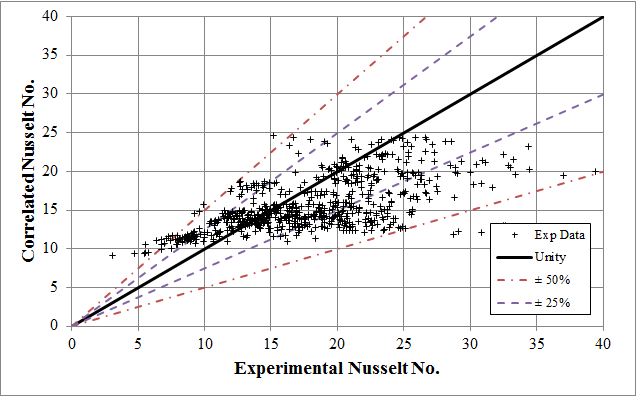
\includegraphics[width=0.8\textwidth]{NuComparisonPondHeatRej.png}
	\caption{Pond heat rejection convection correlation simulated vs.\ experimental Nusselt number comparison}
	\label{fig:Correlation:PondHeatRej:NuComparison}
\end{figure}

From Figure \ref{fig:Correlation:PondHeatRej:NuComparison}, we can see a significant amount of scatter in the data. To give a better indication of how well Equation \ref{eq:Correlation:PondHeatRej:Corr} correlates to the experimental pond heat rejection data, a histogram plot of the percent error can be seen in Figure \ref{fig:Correlation:PondHeatRej:NuComparisonHistogram}. 		
		
\begin{figure}
	\centering
	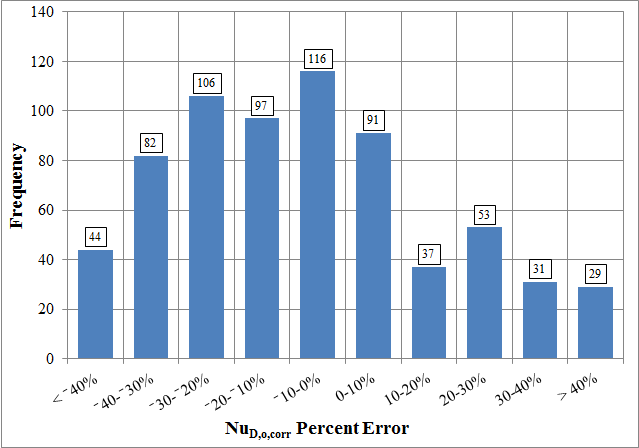
\includegraphics[width=0.8\textwidth]{NuComparisonHistogramPondHeatRej.png}
	\caption{Pond heat rejection convection correlation histogram of simulated vs.\ experimental Nusselt number percent error}
	\label{fig:Correlation:PondHeatRej:NuComparisonHistogram}
\end{figure}

Here again, we can see that the percent error for most of the data set is scattered within $\pm 40\%$ of unity. This result is not ideal, but because the outside convective resistance only makes up a fraction of the total thermal resistance, heat transfer prediction results can still be reasonable.

		
\subsubsection{Experimental vs.\ Simulated Heat Transfer Comparison}
			
In order to compare Equation \ref{eq:Correlation:PondHeatRej:Corr} based on how well heat transfer is predicted, a simulation was set up to compare the simulated heat transfer rate against the experimental heat transfer rate. To do this, the experimental entering fluid temperature, fluid flow rate, SHWE geometry, and surface water temperatures were all input into a model used to determine simulated SHWE heat transfer rate for that given experimental measurement. This model used Equation \ref{eq:Correlation:PondHeatRej:Corr} as the correlation for determining the outside convective thermal resistance as well as the experimental circulating fluid inlet temperature, flow rate, and SWHE coil geometry as model inputs. A plot showing the simulated and experimental heat transfer rates can be seen in Figure \ref{fig:Correlation:PondHeatRej:HTComparison}. 
			
\begin{figure}
	\centering
	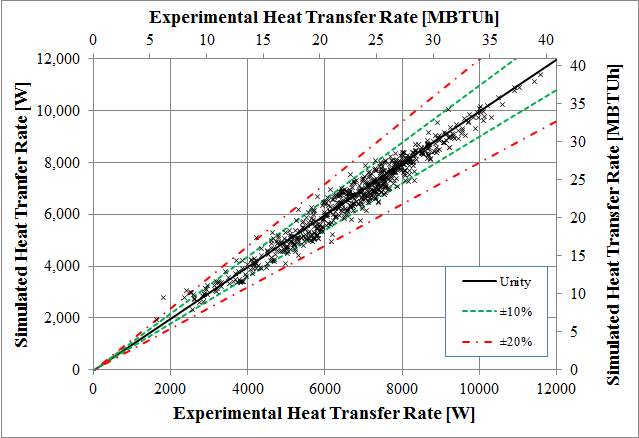
\includegraphics[width=0.8\textwidth]{HTComparisonPondHeatRej.png}
	\caption{Pond heat rejection convection correlation simulated vs.\ experimental heat transfer rates}
	\label{fig:Correlation:PondHeatRej:HTComparison}
\end{figure}

Here, we can see that despite the data scatter seen in Figure \ref{fig:Correlation:PondHeatRej:NuComparison} for the correlated and experimental Nusselt numbers, the heat transfer rate can be predicted quite well. A histogram plot of the simulation vs.\ experimental heat transfer rates can be seen in Figure \ref{fig:Correlation:PondHeatRej:HTComparisonHistogram}. From this plot, we can see that heat transfer percent error is centered around 0\% error with most of the rest of the data within $\pm10\%$ of the experimental data.

\begin{figure}
	\centering
	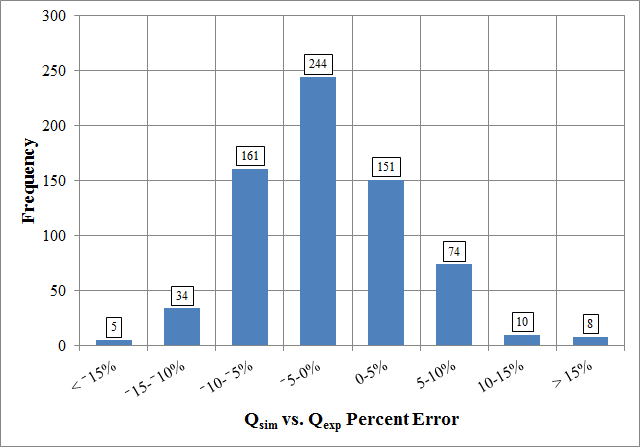
\includegraphics[width=0.8\textwidth]{HTComparisonHistogramPondHeatRej.png}
	\caption{Pond heat rejection convection correlation simulated vs.\ experimental heat transfer rate percent error histogram}
	\label{fig:Correlation:PondHeatRej:HTComparisonHistogram}
\end{figure}

The reason for this behavior is given in Table \ref{tab:ExpResult:PondHeatRej:ThermalPercentage} which shows the average thermal resistance of each thermal resistance component as a percentage of total thermal resistance. From this table we can see that the outside convection thermal resistance only makes up a relatively small portion of the total thermal resistance. On average across the three tube sizes tested, the outside thermal resistance makes up only 28\% of the total thermal resistance. This implies that even given the $\pm40\%$ differences in predicted Nusselt numbers, the total thermal resistance is only expected to be affected by around $\pm11\%$.
	
Table \ref{tab:Correlation:PondHeatRej:StatSummaryTable} summarizes the statistics for how well the Nusselt number and heat transfer results are predicted based on Equation \ref{eq:Correlation:PondHeatRej:Corr}. The key point to note is that despite the Nusselt number RMSE being approximately 27\%, the heat transfer RMSE is considerably better at 6\% due to what was just discussed.

	\begin{table}[h]
		\centering
		\caption{RMSE and MBE statistics for the pond heat rejection convection correlation}
		\label{tab:Correlation:PondHeatRej:StatSummaryTable}
		\begin{tabular}{c c c c}
		\hline
		\multicolumn{2}{c}{Nusselt Number} & \multicolumn{2}{c}{Heat Transfer Rate} \\
		RMSE \% & MBE \% & RMSE \% & MBE \% \\
		\hline\hline
		27.1 & -6.5 & 6.3 & -1.6 \\
		\hline		
		\end{tabular}
	\end{table}
	
\subsection{Pool Heat Rejection Data Convection Correlation}
		
For this data set, the correlation described in Section \ref{subsec:Correlation:PondHeatRej} was taken as the base outside convection correlation. From the base case, this data set was taken and the correlation multiplier was optimized to provide the best fit to the data. It was observed that the data collected in the pool under heat rejection conditions tended to have Nusselt numbers which were much less than the data collected in the pond for the same SWHE geometry. Hence, the convection multiplier will cause the outside Nusselt number to be smaller than it would be if it were in the pond. The correlation developed for the pool heat rejection data can be seen in Equation \ref{eq:Correlation:PoolHeatRej:Corr}.

\begin{equation}
	\mbox{Nu}_{D,o} = 0.573 \cdot \left(5+ 0.0317 \cdot \mbox{Ra}_{D,o}^{* \, 0.333} \cdot \left(\frac{\Delta y}{D_o}\right)^{0.344} \cdot \left(\frac{\Delta x}{D_o}\right)^{0.301}\right)
	\label{eq:Correlation:PoolHeatRej:Corr}
\end{equation}


\subsubsection{Experimental vs.\ Correlated Nusselt Number Comparison}
			
Figure \ref{fig:Correlation:PoolHeatRej:NuComparison} below shows the correlated vs.\ experimental Nusselt number comparison plot. Error bars for $\pm10\%$ and $\pm25\%$ are show also shown. Figure \ref{fig:Correlation:PoolHeatRej:NuComparisonHistogram} shows a histogram plot of the correlated vs.\ experimental percent error for Equation \ref{eq:Correlation:PoolHeatRej:Corr}.
			
\begin{figure}
	\centering
	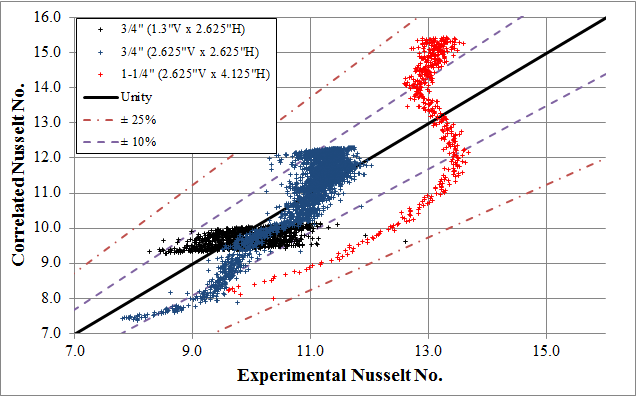
\includegraphics[width=0.8\textwidth]{NuComparisonPoolHeatRej.png}
	\caption{Pool heat rejection convection correlation simulated vs.\ experimental Nusselt number comparison}
	\label{fig:Correlation:PoolHeatRej:NuComparison}
\end{figure}

\begin{figure}
	\centering
	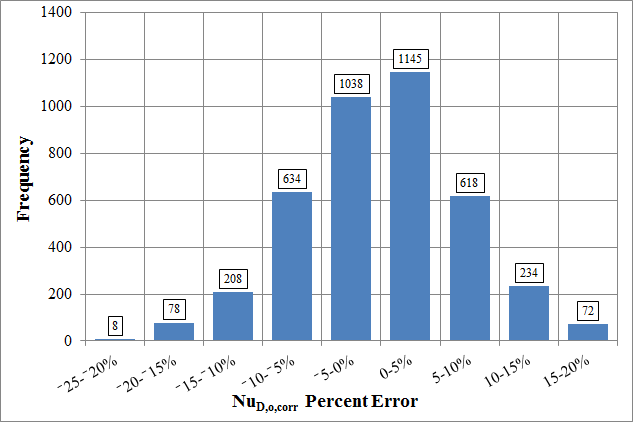
\includegraphics[width=0.8\textwidth]{NuComparisonHistogramPoolHeatRej.png}
	\caption{Pool heat rejection convection correlation simulated vs.\ experimental Nusselt number comparison histogram}
	\label{fig:Correlation:PoolHeatRej:NuComparisonHistogram}
\end{figure}
			
From the two figures above we can see that the 3/4 in.\ (19 mm) data is predicted reasonably well by Equation \ref{eq:Correlation:PoolHeatRej:Corr}. However, the 1-1/4 in.\ (32 mm) data shows trends that are not captured by the convection correlation. The 1-1/4 in.\ (32 mm) data tends to be under predicted by the convection correlation in the lower range of Nusselt numbers, then over predicted at higher Nusselt numbers. The reason for this can be observed in Figure \ref{fig:ExpResult:HeatRej:PoolData:Pool_125D_4125H_2626V_HeatRej}, where the experimental Nusselt number increases, as expected with increasing Rayleigh number. However, something begins occurring at $Ra_D^*=3.5\cdot10^7$ when the Nusselt numbers begin decreasing with increases in Rayleigh numbers. The reason for this non-monotonic behavior is not fully understood, but the author theorizes that it is due to the constrained nature of the pool in which the experiments were performed.
			
\subsubsection{Experimental vs.\ Simulated Heat Transfer Comparison}
			
Comparing the heat transfer results for the pool heat rejection data, we can again see that the correlation shown in Equation \ref{eq:Correlation:PoolHeatRej:Corr} predicts the heat transfer reasonably well. Figure \ref{fig:Correlation:PoolHeatRej:HTComparison} shows the simulated vs.\ experimental heat transfer rate comparison, and Figure \ref{fig:Correlation:PoolHeatRej:HTComparisonHistogram} shows the histogram of the simulated vs.\ experimental percent error.
			
\begin{figure}
	\centering
	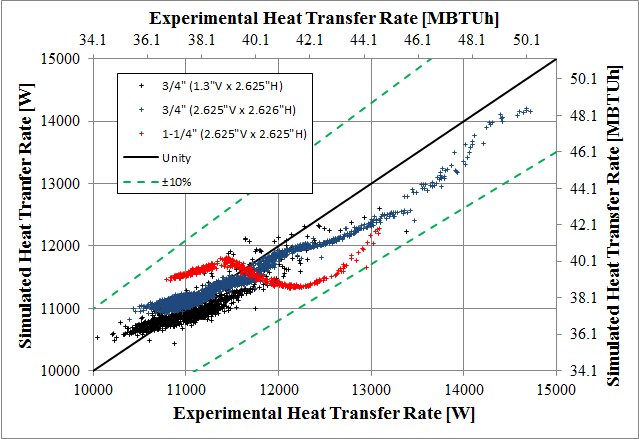
\includegraphics[width=0.8\textwidth]{HTComparisonPoolHeatRej.png}
	\caption{Pool heat rejection convection correlation simulated vs.\ experimental heat transfer rates}
	\label{fig:Correlation:PoolHeatRej:HTComparison}
\end{figure}


\begin{figure}
	\centering
	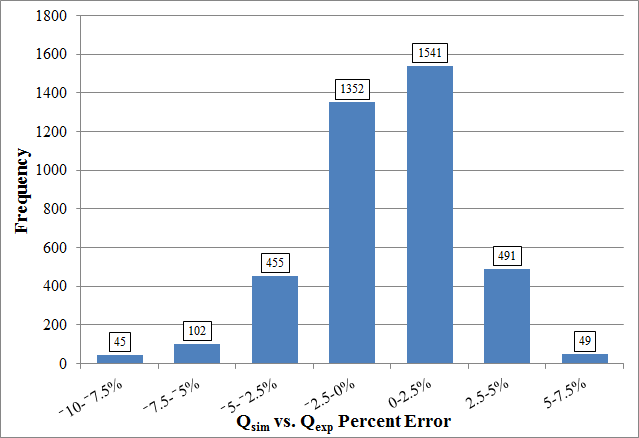
\includegraphics[width=0.8\textwidth]{HTComparisonHistogramPoolHeatRej.png}
	\caption{Pool heat rejection convection correlation simulated vs.\ experimental heat transfer rate histogram of percent error}
	\label{fig:Correlation:PoolHeatRej:HTComparisonHistogram}
\end{figure}	

From these figures, we can see that using Equation \ref{eq:Correlation:PoolHeatRej:Corr} to predict the outside convection resistance correlates nearly all of the experimental data within $\pm10\%$. For the given data, this is sightly better than the results for the pond heat rejection.


Table \ref{tab:Correlation:PoolHeatRej:StatSummaryTable} shows the summary of statisitcs to quantify how well Equation \ref{eq:Correlation:PoolHeatRej:Corr} predicts the outside convection resistance for the pool heat rejection data.	

	\begin{table}[h]
		\centering
		\caption{RMSE and MBE statistics for the pool heat rejection convection correlation}
		\label{tab:Correlation:PoolHeatRej:StatSummaryTable}
		\begin{tabular}{c c c c}
		\hline
		\multicolumn{2}{c}{Nusselt Number} & \multicolumn{2}{c}{Heat Transfer Rate} \\
		RMSE \% & MBE \% & RMSE \% & MBE \% \\
		\hline\hline
		6.9 & 0.0 & 2.5 & -0.1 \\
		\hline		
		\end{tabular}
	\end{table}	


\subsection{Heat Rejection Convection Correlation Comparison}
\label{subsec:Correlation:HeatRejComparison}

To compare the two correlations described above, the correlations were compared against experimental data for each data set. Due to the limited number of overlapping geometrical configurations, the 3/4 in.\ (19 mm) 2.625 in.\ H x 2.625 in.\ V (67 mm x 67 mm) data was selected for comparison purposes. Figure \ref{fig:Correlation:HeatRejComparison:NuCompare} shows the experimental data, and the convection correlations for the specific SWHE geometry plotted together. From the figure, we can see that the Nusselt number for the pool data is considerably lower than the pond data. This is reflected in the pool convection correlation.

\begin{figure}
	\centering
	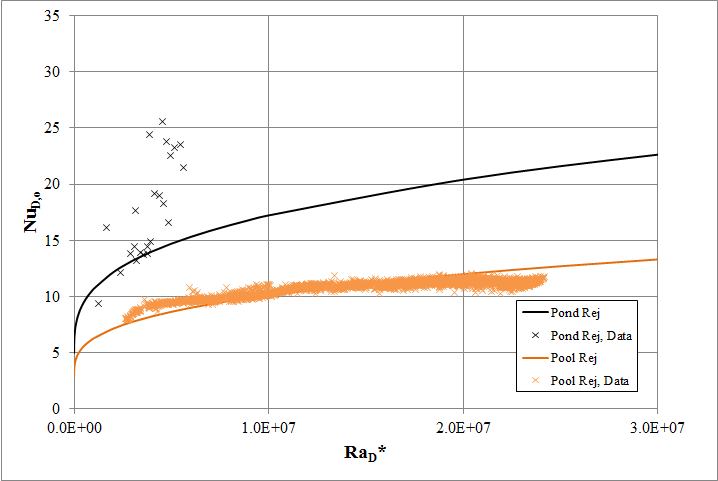
\includegraphics[width=0.8\textwidth]{NuCompareHeatRej.png}
	\caption{Heat rejection convection correlation Nusselt number comparison}
	\label{fig:Correlation:HeatRejComparison:NuCompare}
\end{figure}
			
\subsection{Pool Heat Extraction Data Convection Correlation}
\label{subsec:Correlation:PoolHeatExtr}

Because the pool heat extraction data was selected as the base data set for heat extraction, the base convection correlation will be developed in this section. As a continuation of the discussion in Section \ref{subsec:ExpResult:HeatExtr:PoolData}, the heat extraction data is very sensitive near the surface water maximum density point. This was described previously regarding the trends shown when the convective plume flow direction changes from downward flow to upward flow. 

Figure \ref{fig:Correlation:PoolHeatExtr:NuVsRa} below show the data from Figures \ref{fig:ExpResult:HeatExtr:PoolData:Pool_075D_2625H_15V_HeatExtr}, \ref{fig:ExpResult:HeatExtr:PoolData:Pool_075D_2625H_2626V_HeatExtr}, and \ref{fig:ExpResult:HeatExtr:PoolData:Pool_125D_4125H_2626V_HeatExtr} combined into a single figure. In order to organize the data and distinguish between the data which likely to have downward flow vs.\ data that is likely to have upward flow, the Rayleigh number was multiplied by the flow direction scalar $\delta$ based on the conditions indicated in Table \ref{tab:Correlation:PoolHeatExtr:FDS}. A positive $\delta$ indicates downward plume flow, while a negative $\delta$ indicates an upward plume flow. This data can be seen in Figure \ref{fig:Correlation:PoolHeatExtr:NuVsRaPlusDelta} where  $\delta$ is multiplied by the modified Rayleigh number. 

\begin{figure}
	\centering
	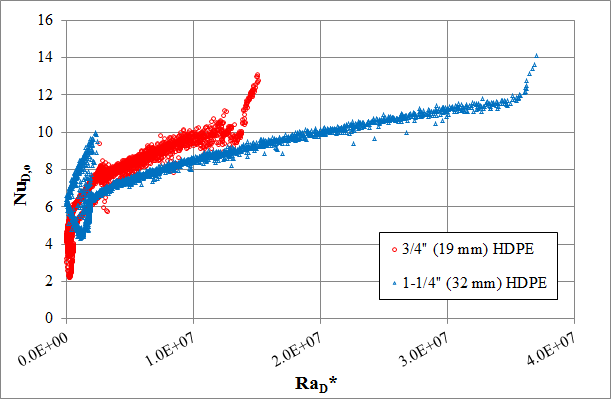
\includegraphics[width=0.8\textwidth]{NuVsRaPoolHeatExtr.png}
	\caption{Nusselt vs.\ modified Rayleigh number plot of combined pool heat extraction data}
	\label{fig:Correlation:PoolHeatExtr:NuVsRa}
\end{figure}

\begin{table}[h]
	\centering
	\caption{Flow direction scalar}
	\label{tab:Correlation:PoolHeatExtr:FDS}
	\begin{tabular}{r c r c l}
	\multirow{2}{*}{$\delta = \bigg\{$} & 1 if: & $\rho_{sw-T,film,o}$ & $<$ & $\rho_{sw-T,sw}$ \\
	 & -1 if: & $\rho_{sw-T,film,o}$ & $>$ & $\rho_{sw-T,sw}$ \\
	\end{tabular}
\end{table}
		
\begin{figure}
	\centering
	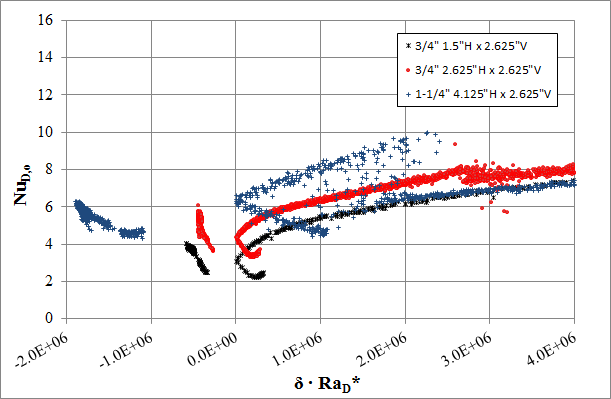
\includegraphics[width=0.8\textwidth]{NuVsRaPoolHeatExtrPlusDelta.png}
	\caption{Nusselt vs.\ flow direction modified Rayleigh number plot of combined pool heat extraction data with flow direction scalar}
	\label{fig:Correlation:PoolHeatExtr:NuVsRaPlusDelta}
\end{figure}

In Figure \ref{fig:Correlation:PoolHeatExtr:NuVsRaPlusDelta} we see some of the data near the lowest Nusselt number that has been reflected about $Ra_D^*=0$ by the flow direction scalar. For the 3/4 in.\ (19 mm) data, the data affected by this flow direction change go from $Ra_D^*=0$ to approximately $Ra_D^*=5\cdot10^5$. The 1-1/4 in.\ (32 mm) data is affected from $Ra_D^*=0$ up to approximately $Ra_D^*=2\cdot10^6$, however, there is still some scatter in the data above $Ra_D^*=2\cdot10^6$.

Because the data has been shown to be very sensitive near the surface water maximum density point, it is very difficult to accurately correlate the data in this region. As is the case with the 1-1/4 in.\ (32 mm) data, and as will be shown in the next section for the 3/4 in.\ (19 mm) pond heat extraction data, Nusselt number experimental data taken in this region can give randomized results. As a result of this sensitivity, the data for the 3/4 in.\ (19 mm) below $Ra_D^*=1\cdot10^6$ and the 1-1/4 in.\ (32 mm) data below $Ra_D^*=3\cdot10^6$ have been omitted from use in the correlation development. Below these points, due to the highly random data, a constant Nusselt number value will be recommended.

Equation \ref{eq:Correlation:PoolHeatExtr:Corr} is the equation that was optimized to fit the pool heat extraction base data set. The correlation's range of applicability can be seen below in Table \ref{tab:Correlation:PoolHeatExtr:RangeOfApp}.

\begin{equation}
	\mbox{Nu}_{D,o} = 0.87 \cdot \left(5.75 + 0.00971 \cdot \mbox{Ra}_{D,o}^{* \, 0.333} \cdot \left(\frac{\Delta y}{D_o}\right)^{0.929}\right)
	\label{eq:Correlation:PoolHeatExtr:Corr}
\end{equation}

	\begin{table}[h]
		\centering
		\caption[Range of applicability for pool heat extraction correlation]{Range of applicability for each parameter in Equation \ref{eq:Correlation:PoolHeatExtr:Corr}}
		\label{tab:Correlation:PoolHeatExtr:RangeOfApp}
		\begin{tabular}{r c c c l}
		$1.0\cdot10^6$ & $\le$ &  $Ra_{D,o}^*$ & $\le$  & $4.0\cdot10^7$ \\
		1.3 in.\ (33 mm) & $\le$ & $\Delta y$ & $\le$ & 2.625 in.\ (67 mm) \\
		2.625 in.\ (67 mm) & $\le$ & $\Delta x$ & $\le$ & 4.125 in.\ (105 mm) \\
		1.05 in.\ (27 mm) & $\le$ &  $D_o$ &  $\le$ & 1.66 in.\ (42 mm) \\
		0.85 in.\ (22 mm) & $\le$ &  $D_i$ &  $\le$ & 1.36 in.\ (36 mm) \\
		\multicolumn{5}{c}{L = 500 ft.\ (153 m)} \\
		\end{tabular}
	\end{table}
	
For values of $Ra_D^*$ less than $1\cdot10^6$ for 3/4 in.\ (19 mm) pipes, and $Ra_D^*$ less than $3\cdot10^6$ for 1-1/4 in.\ (32 mm) pipes, a constant value of $Nu_{D,o}=5$ is used. This number represents a mean value for Nusselt number which can be expected in this range of Rayleigh numbers.

\subsubsection{Experimental vs.\ Correlated Nusselt Number Comparison}

Figure \ref{fig:Correlation:PoolHeatExtr:NuComparison} shows the experimental vs.\ correlated Nusselt number comparison for this data set. Figure \ref{fig:Correlation:PoolHeatExtr:NuComparisonHistogram} shows the histogram plot of the experimental vs.\ correlated Nusselt number percent error. The histogram shows that the percent error is skewed left into negative percent errors. This indicates that the correlation is under predicting the experimental results to a certain degree.

\begin{figure}
	\centering
	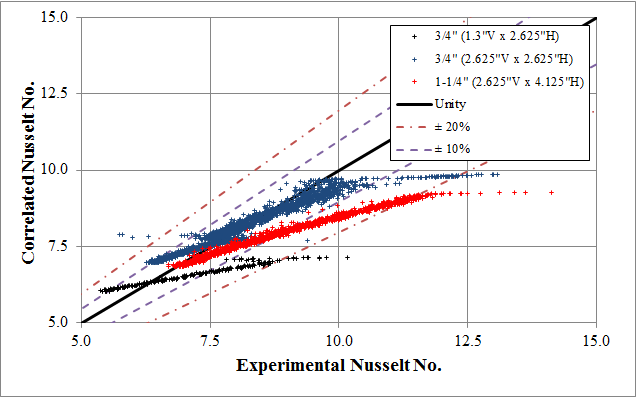
\includegraphics[width=0.8\textwidth]{NuComparisonPoolHeatExtr.png}
	\caption{Pool heat extraction convection correlation simulated vs.\ experimental Nusselt number comparison}
	\label{fig:Correlation:PoolHeatExtr:NuComparison}
\end{figure}

		
\begin{figure}
	\centering
	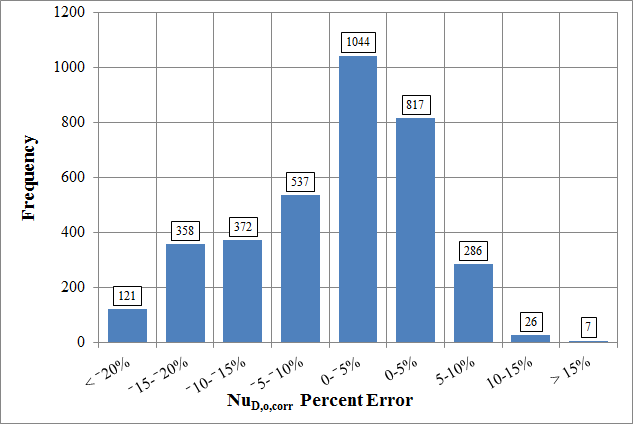
\includegraphics[width=0.8\textwidth]{NuComparisonHistogramPoolHeatExtr.png}
	\caption{Pool heat extraction convection correlation histogram of simulated vs.\ experimental Nusselt number percent error}
	\label{fig:Correlation:PoolHeatExtr:NuComparisonHistogram}
\end{figure}

In Figure \ref{fig:Correlation:PoolHeatExtr:NuComparison} we can see towards the right side of each data set that there is a small band of data that trails off away from the rest of the data. This small band of trailing data is data that was recorded during the initial startup period of the experiments. This data was recorded during the time when initial systems transients were still settling.

Another trend worth noting is the fact that both 3/4 in.\ (19 mm) data sets are mostly centered around the `unity' line. This implies that over the range data, the correlation will predict Nusselt number values that will be centered around the actual value. However, for the 1-1/4 in.\ data, the correlation tends to under predict the Nusselt number by around 0-20\% over the range of experimental data. The reason for this is currently unknown.
			
\subsubsection{Experimental vs.\ Simulated Heat Transfer Comparison}

Figure \ref{fig:Correlation:PoolHeatExtr:HTComparison} shows the simulated vs.\ experimental heat transfer rate comparison for pool heat extraction data set using Equation \ref{eq:Correlation:PoolHeatExtr:Corr} as the outside convection correlation. Figure \ref{fig:Correlation:PoolHeatExtr:HTComparisonHistogram} shows the histogram plot of the percent error between the experimental and simulated results.

We can see that the 3/4 in.\ (19 mm) 2.625 in.\ V x 2.625 in.\ H (67 mm x 67 mm) results  tend to be similar to the Nusselt number results shown in Figure \ref{fig:Correlation:PoolHeatExtr:NuComparison}. The other two data sets, however, tend to have the magnitude of the heat transfer under predicted by up to 10\%. This occurs due to the outside Nusselt number being incorrectly predicted by Equation \ref{eq:Correlation:PoolHeatExtr:Corr}. Even given this, heat transfer is predicted reasonably well at lower heat transfer rates. At higher heat transfer rates, the simulated heat transfer rate deviates from the experimental value by up to 10\%.

	\begin{figure}
		\centering
		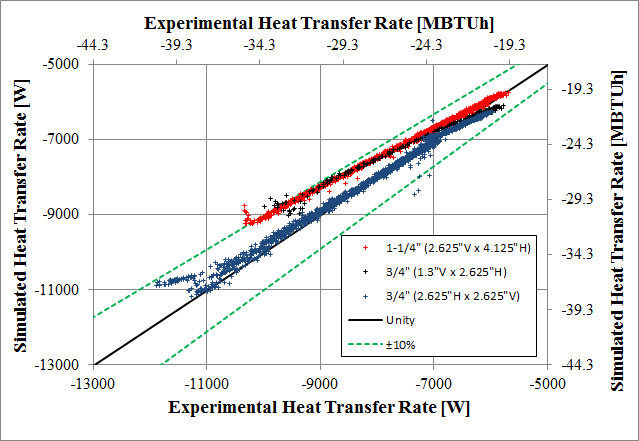
\includegraphics[width=0.8\textwidth]{HTComparisonPoolHeatExtr.png}
		\caption{Pool heat extraction convection correlation simulated vs.\ experimental heat transfer rates}
		\label{fig:Correlation:PoolHeatExtr:HTComparison}
	\end{figure}


	\begin{figure}
		\centering
		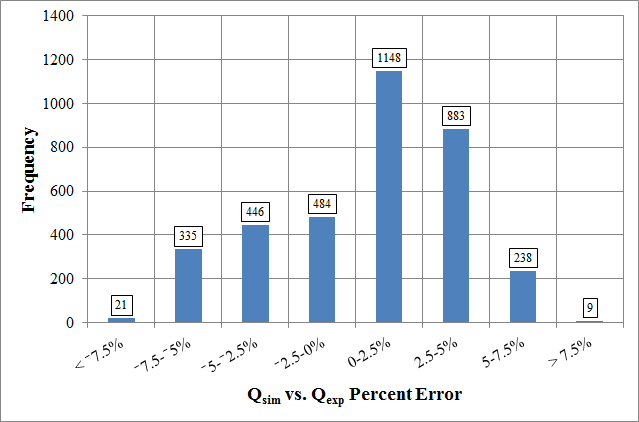
\includegraphics[width=0.8\textwidth]{HTComparisonHistogramPoolHeatExtr.png}
		\caption{Pool heat extraction convection correlation simulated vs.\ experimental heat transfer rate histogram of percent error}
		\label{fig:Correlation:PoolHeatExtr:HTComparisonHistogram}
	\end{figure}

Table \ref{tab:Correlation:PoolHeatExtr:StatSummaryTable} shows the statistical measures used to quantify how well the correlation predicts Nusselt number, and how how well the simulation, using Equation \ref{eq:Correlation:PoolHeatExtr:Corr} to predict outside Nusselt number, predicts heat transfer rate. 
	
	\begin{table}[h]
		\centering
		\caption{RMSE and MBE statistics for the pool heat extraction convection correlation}
		\label{tab:Correlation:PoolHeatExtr:StatSummaryTable}
		\begin{tabular}{c c c c}
		\hline
		\multicolumn{2}{c}{Nusselt Number} & \multicolumn{2}{c}{Heat Transfer Rate} \\
		RMSE \% & MBE \% & RMSE \% & MBE \% \\
		\hline\hline
		9.1 & -4.5 & 4.1 & -2.0 \\
		\hline		
		\end{tabular}
	\end{table}	


\subsection{Pond Heat Extraction Data Convection Correlation}

To show the sensitivity of the pond heat extraction data near the surface water maximum density point, the flow direction scalar as shown in Table \ref{tab:Correlation:PoolHeatExtr:FDS} is again applied to this data set. This can be seen Figure \ref{fig:Correlation:PondHeatExtr:NuVsRaPlusDelta} where data from $Ra_D^* = 0$ to $Ra_D^* = 1 \cdot 10^6$ is reflected about $Ra_D^* = 0$. 

	\begin{figure}
		\centering
		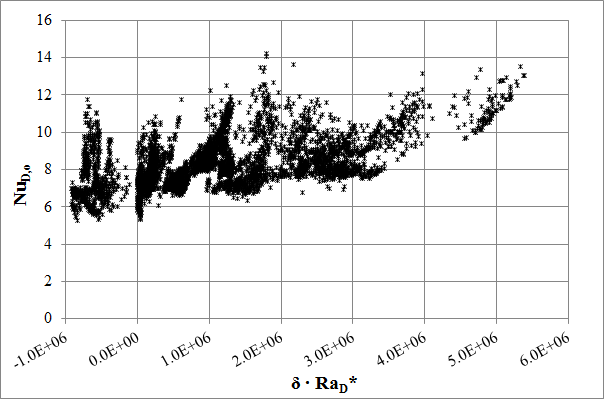
\includegraphics[width=0.8\textwidth]{NuVsRaPondHeatExtrPlusDelta.png}
		\caption{Nusselt vs.\ modified Rayleigh number plot of combined pond heat extraction data with flow direction scalar}
		\label{fig:Correlation:PondHeatExtr:NuVsRaPlusDelta}
		\end{figure}
		
As was the case with the previous data set, this data shows highly random and data near the maximum density point. As a result of this, the data from $Ra_D^* = 0$ to $Ra_D^* = 1 \cdot 10^6$ is not used in the development of the convection correlation.
		
Because this is the alternative data set for heat extraction, the correlation developed in the previous section will be used for the pond heat extraction data correlation. Because the pool data tended to under predict the pond data during heat extraction conditions, the multiplier was optimized to scale the correlation shown in Equation \ref{eq:Correlation:PoolHeatExtr:Corr} up to best fit the pond heat extraction data. Equation \ref{eq:Correlation:PondHeatExtr:Corr} below shows this correlation.

	\begin{equation}
		\mbox{Nu}_{D,o} = 5.75 + 0.00971 \cdot \mbox{Ra}_{D,o}^{* \, 0.333} \cdot \left(\frac{\Delta y}{D_o}\right)^{0.929}
	\label{eq:Correlation:PondHeatExtr:Corr}
	\end{equation}
	
\subsubsection{Experimental vs.\ Correlated Nusselt Number Comparison}

Figure \ref{fig:Correlation:PondHeatExtr:NuComparison} shows the correlated vs.\ experimental Nusselt number comparison plot for the pond heat extraction data as correlated by Equation \ref{eq:Correlation:PondHeatExtr:Corr}. Also shown are the $\pm10\%$ and $\pm25\%$ error bars. From the plot, it is obvious that there are conditions occurring in the experiment which were not accounted for the correlation. This experiment was performed outdoors in a pond which was exposed to the weather elements. Some theoretical possibilities for conditions affecting the data are wind or underwater currents. Wave action causing the support platform to move excessively could also have caused the convective boundary layers to be disturbed, thus giving the effect of lower outside convective resistance. These are all theoretical possibilities, however, the actual reason for the discrepancy is unknown at this time. By comparison, a similar behavior was observed for the pond heat rejection data in Figure \ref{fig:Correlation:PondHeatRej:NuComparison}. 

	\begin{figure}
		\centering
		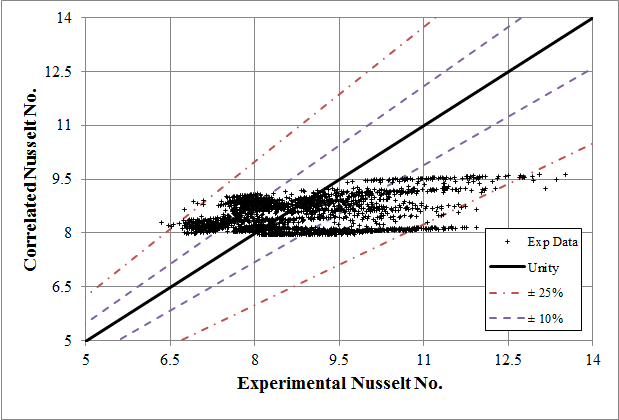
\includegraphics[width=0.8\textwidth]{NuComparisonPondHeatExtr.png}
		\caption{Pond heat extraction convection correlation simulated vs.\ experimental Nusselt number comparison}
		\label{fig:Correlation:PondHeatExtr:NuComparison}
	\end{figure}
	
Figure \ref{fig:Correlation:PondHeatExtr:HTComparisonHistogram} shows a histogram plot of correlated vs.\ experimental Nusselt number percent error. From this we see that at the very least, the data is centered around the 0\% error with error mostly bounded with in $\pm30$\% error. The result is not ideal, but over the range of data, the correlated Nusselt numbers will be centered around the experimental data.
	
	\begin{figure}
		\centering
		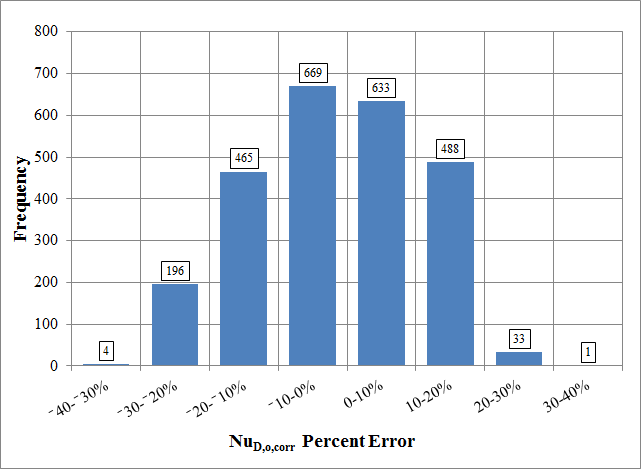
\includegraphics[width=0.8\textwidth]{NuComparisonHistogramPondHeatExtr.png}
		\caption{Pond heat extraction convection correlation simulated vs.\ experimental Nusselt number comparison histogram}
		\label{fig:Correlation:PondHeatExtr:NuComparisonHistogram}
	\end{figure}
			
\subsubsection{Experimental vs.\ Simulated Heat Transfer Comparison}
		
Figure \ref{fig:Correlation:PondHeatExtr:HTComparison} shows how well the simulation using the correlation described in Equation \ref{eq:Correlation:PondHeatExtr:Corr} for the outside Nusselt number predicts the SWHE heat transfer rate. Figure \ref{fig:Correlation:PondHeatExtr:HTComparisonHistogram} shows a histogram plot of the heat transfer rate percent error. Here again we see that although the Nusselt number is not correlated perfectly, the heat transfer rates are nearly all predicted to within 10\% of experimental data.
		
\begin{figure}
	\centering
	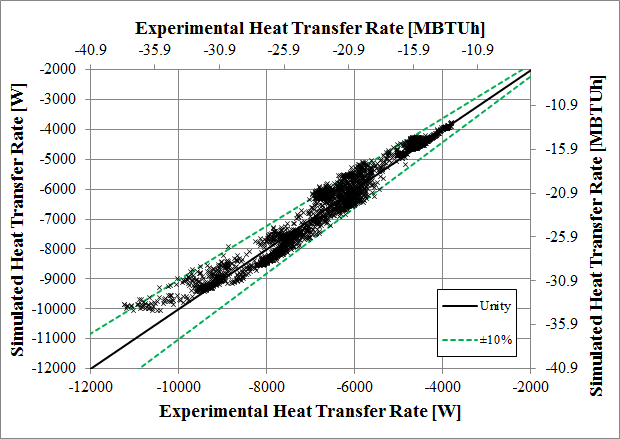
\includegraphics[width=0.8\textwidth]{HTComparisonPondHeatExtr.png}
	\caption{Pond heat extraction convection correlation simulated vs.\ experimental heat transfer rates}
	\label{fig:Correlation:PondHeatExtr:HTComparison}
\end{figure}

\begin{figure}
	\centering
	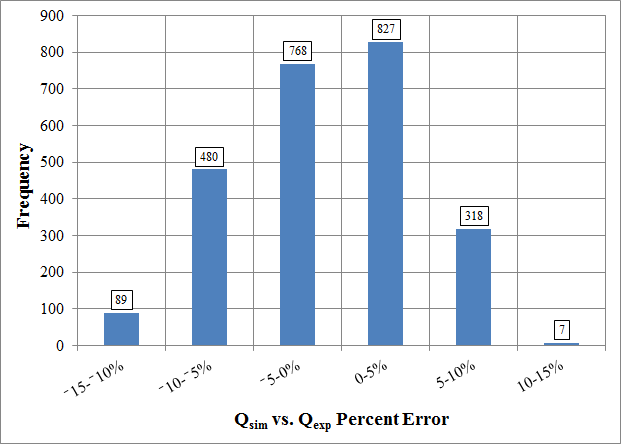
\includegraphics[width=0.8\textwidth]{HTComparisonHistogramPondHeatExtr.png}
	\caption{Pond heat extraction convection correlation simulated vs.\ experimental heat transfer rate histogram of percent error}
	\label{fig:Correlation:PondHeatExtr:HTComparisonHistogram}
\end{figure}
	
Table \ref{tab:Correlation:PondHeatExtr:StatSummaryTable} shows the RMSE and MBE statistics to quantify how well Equation \ref{eq:Correlation:PondHeatExtr:Corr} predicts the Nusselt number and heat transfer rates of the pond heat extraction data. 

	\begin{table}[h]
		\centering
		\caption{RMSE and MBE statistics for the pond heat extraction convection correlation}
		\label{tab:Correlation:PondHeatExtr:StatSummaryTable}
		\begin{tabular}{c c c c}
		\hline
		\multicolumn{2}{c}{Nusselt Number} & \multicolumn{2}{c}{Heat Transfer Rate} \\
		RMSE \% & MBE \% & RMSE \% & MBE \% \\
		\hline\hline
		12.2 & -1.8 & 5.0 & -0.8 \\
		\hline		
		\end{tabular}
	\end{table}

\subsection{Heat Extraction Convection Correlation Comparison}
\label{subsec:Correlation:HeatExtrComparison}

To compare the two correlations described above for heat extraction, the correlations were compared against experimental data for each data set. Again, due to the limited number of overlapping geometrical configurations, the 3/4 in.\ (19 mm) 2.625 in.\ H x 2.625 in.\ V (67 mm x 67 mm) data was selected for comparison purposes. Figure \ref{fig:Correlation:HeatExtrComparison:NuCompare} shows the experimental data, and the convection correlations for the specific SWHE geometry plotted together. From the figure, we can see that the Nusselt number for the pool data is lower than the data from the pond. 


\begin{figure}
	\centering
	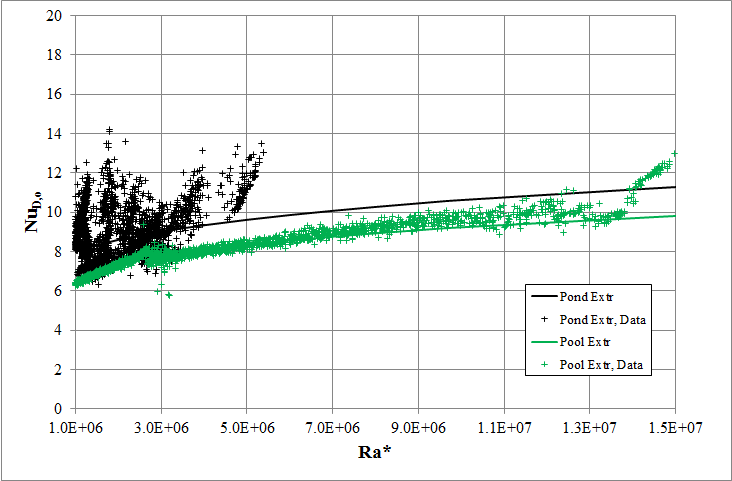
\includegraphics[width=0.8\textwidth]{NuCompareHeatExtr.png}
	\caption{Heat extraction convection correlation Nusselt number comparison}
	\label{fig:Correlation:HeatExtrComparison:NuCompare}
\end{figure}

\section{Churchill-Chu Correlation Comparison}
\label{sec:Corrleation:Churchill}

Up until this point, there have been no comparisons of the convection correlation derived in this work against standard correlations for straight pipes, which is what has  been used for surface water heat exhangers prior to this work \citep{Chiasson1999}. In this section, the experimental data is compared against the \cite{ChurchillChu1975} correlation for free convection from a horizontal cylinder. The results are compared and a summarized to give the reader another means whereby to compare the current work.

\subsection{Pond Heat Rejection Data Comparison}
\label{Correlation:Churchill:PondHR}

For the pond heat rejection data, some benefits are realized when comparing the Nusselt number RMSE and MBE. For the \cite{ChurchillChu1975} correlation, RMSE percent error was 41.9\% for the \cite{ChurchillChu1975} correlation vs.\ the 27.1\% for the correlation presented during this work. MBE is however, slightly better going to -5.0\% for the \cite{ChurchillChu1975} correlation vs.\ -6.5\% for the present correlation. Figure \ref{fig:Correlation:Churchill:NuPondHR} shows the Nusselt number as calculated by the \cite{ChurchillChu1975} correlation against the experimentally derived pond heat rejection Nusselt numbers. Figure \ref{fig:Correlation:PondHeatRej:NuComparison} can be compared for reference to the current correlation.

\begin{figure}
	\centering
	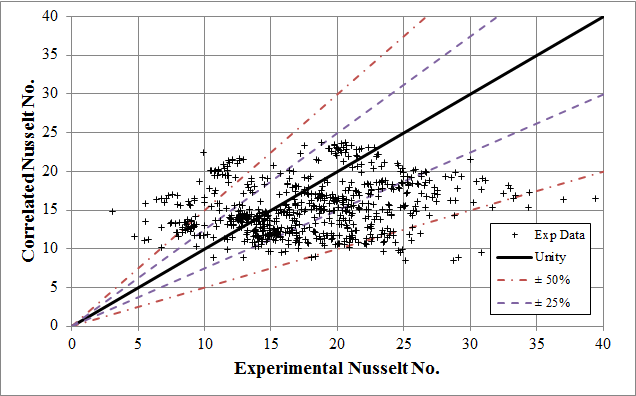
\includegraphics[width=0.8\textwidth]{NuChurchillPondHR.png}
	\caption{Nusselt number comparison for the Churchill-Chu correlation vs.\ experimental pond heat rejection data}
	\label{fig:Correlation:Churchill:NuPondHR}
\end{figure}

The difference in Nusselt number has a much smaller effect on heat transfer when the \cite{ChurchillChu1975} correlation is used in a simulation to calculate the heat transfer rates. For the \cite{ChurchillChu1975} correlation, RMSE percent error was 7.1\% when by comparison the correlation presented during this work had an RMSE percent error of 6.3\%. Figure \ref{fig:Correlation:Churchill:HTPondHR} show the heat transfer results for the simulation vs.\ the experimentally derived pond heat rejection data. For comparison, Figure \ref{fig:Correlation:PondHeatRej:HTComparison} can be referenced for comparison of the correlation presented in this work.

\begin{figure}
	\centering
	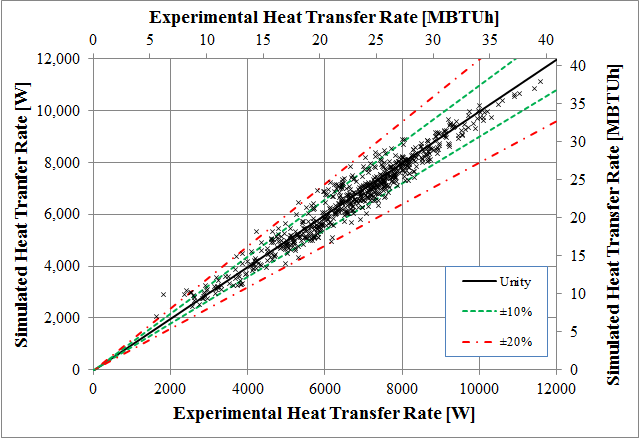
\includegraphics[width=0.8\textwidth]{HTChurchillPondHR.png}
	\caption{Heat transfer rate comparison for the Churchill-Chu correlation vs.\ experimental pond heat rejection data}
	\label{fig:Correlation:Churchill:HTPondHR}
\end{figure}

\subsection{Pool Heat Rejection Data Comparison}
\label{Correlation:Churchill:PoolHR}

For the pool heat rejection data, the benefits of the current work are much more pronounced when compared to the \cite{ChurchillChu1975} convection correlation. Figure \ref{fig:Correlation:Churchill:NuPoolHR} shows the Nusselt number comparison for the \cite{ChurchillChu1975} correlation vs.\ the experimentally derived pool heat rejection data. The reader may reference Figure \ref{fig:Correlation:PoolHeatRej:NuComparison} for the Nusselt number correlation from the present work. The correlation by \cite{ChurchillChu1975} showed a Nusselt number RMSE percent error of 92.6\% whereas the current correlation showed a 6.9\% error for the same data.

\begin{figure}
	\centering
	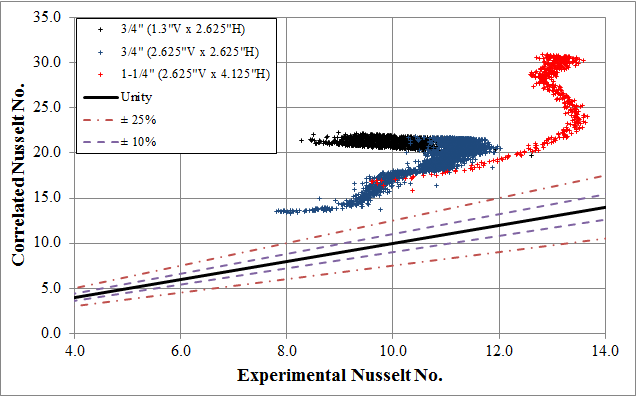
\includegraphics[width=0.8\textwidth]{NuChurchillPoolHR.png}
	\caption{Nusselt number comparison for the Churchill-Chu correlation vs.\ experimental pool heat rejection data}
	\label{fig:Correlation:Churchill:NuPoolHR}
\end{figure}

Figure \ref{fig:Correlation:Churchill:HTPoolHR} shows the heat transfer comparison results when the \cite{ChurchillChu1975} correlation is utilized in the simulated comparison of the experimental data. The reader can refer to Figure \ref{fig:Correlation:PoolHeatRej:HTComparison} for comparison against the current work. For this case, the RMSE percent error for the heat transfer error is 15.4\% whereas the correlation presented in this work is 2.5\%. We can also see that the correlation over predicts Nusselt number, which is reflected in the over prediction of the heat transfer results.

\begin{figure}
	\centering
	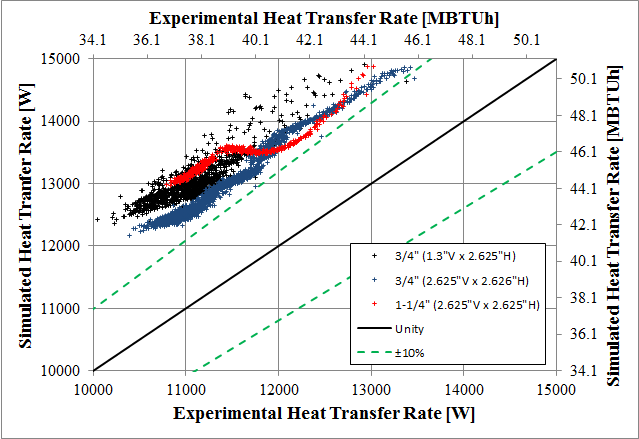
\includegraphics[width=0.8\textwidth]{HTChurchillPoolHR.png}
	\caption{Heat transfer rate comparison for the Churchill-Chu correlation vs.\ experimental pool heat rejection data}
	\label{fig:Correlation:Churchill:HTPoolHR}
\end{figure}

\subsection{Pond Heat Extraction Data Comparison}
\label{Correlation:Churchill:PondHE}

For the pond heat extraction data, we can see that the \cite{ChurchillChu1975} correlation tends to again over predict the Nusselt number. This can be seen in Figure \ref{fig:Correlation:Churchill:NuPondHE}. Figure \ref{fig:Correlation:PondHeatExtr:NuComparison} can also be referenced by the reader to compare against the Nusselt number predictions for the current correlation. For the \cite{ChurchillChu1975} correlation, the RMSE percent error is 44.9\% whereas for the correlation developed in this work, the RMSE percent error is 12.2\%.

\begin{figure}
	\centering
	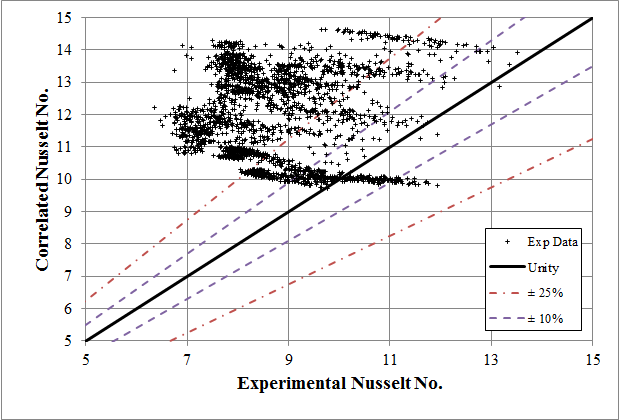
\includegraphics[width=0.8\textwidth]{NuChurchillPondHE.png}
	\caption{Nusselt number comparison for the Churchill-Chu correlation vs.\ experimental pond heat extraction data}
	\label{fig:Correlation:Churchill:NuPondHE}
\end{figure}

The discrepancy in Nusselt number over prediction is reflected again in the simulated heat transfer comparison results. Figure \ref{fig:Correlation:Churchill:HTPondHE} shows the heat transfer comparison against the pond heat extraction data. Figure \ref{fig:Correlation:PondHeatExtr:HTComparison} can also be referenced for comparison against the correlation presented in this work. For the \cite{ChurchillChu1975} correlation, the RMSE percent error is 11.8\% whereas for the current correlation same error is 5.0\%.

\begin{figure}
	\centering
	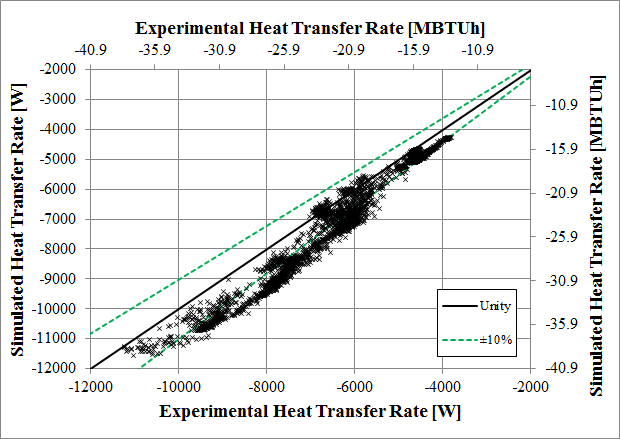
\includegraphics[width=0.8\textwidth]{HTChurchillPondHE.png}
	\caption{Heat transfer rate comparison for the Churchill-Chu correlation vs.\ experimental pond heat extraction data}
	\label{fig:Correlation:Churchill:HTPondHE}
\end{figure}

\subsection{Pool Heat Extraction Data Comparison}
\label{Correlation:Churchill:PoolHE}

For the pool heat extraction data, we again see that the \cite{ChurchillChu1975} correlation over predicts the experimental data. This can be seen in Figure \ref{fig:Correlation:Churchill:NuPoolHE}. Figure \ref{fig:Correlation:PoolHeatExtr:NuComparison} can be referenced for comparison to the current convection correlation. The Nusselt number RMSE percent error for the \cite{ChurchillChu1975} correlation  is 99.6\% whereas the same error for the current correlation is 9.1\%.

\begin{figure}
	\centering
	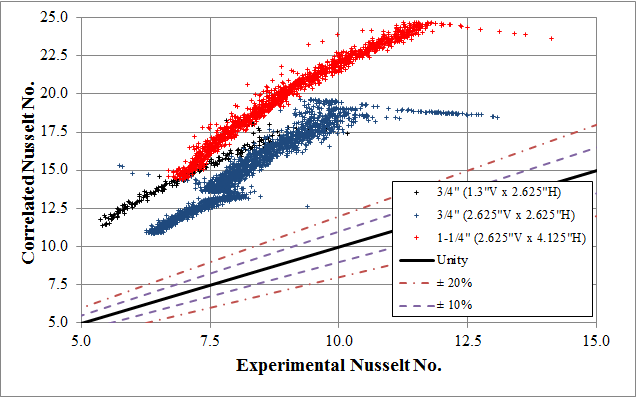
\includegraphics[width=0.8\textwidth]{NuChurchillPoolHE.png}
	\caption{Nusselt number comparison for the Churchill-Chu correlation vs.\ experimental pool heat extraction data}
	\label{fig:Correlation:Churchill:NuPoolHE}
\end{figure}

Figure \ref{fig:Correlation:Churchill:HTPoolHE} shows the simulated heat transfer comparison for the \cite{ChurchillChu1975} correlation. By comparison, Figure \ref{fig:Correlation:PoolHeatExtr:HTComparison} can be referenced for the heat transfer comparison against the current correlation. The heat transfer RMSE percent error for the \cite{ChurchillChu1975} correlation is 21.6\% whereas the same error for the current correlation is 4.1\%.

\begin{figure}
	\centering
	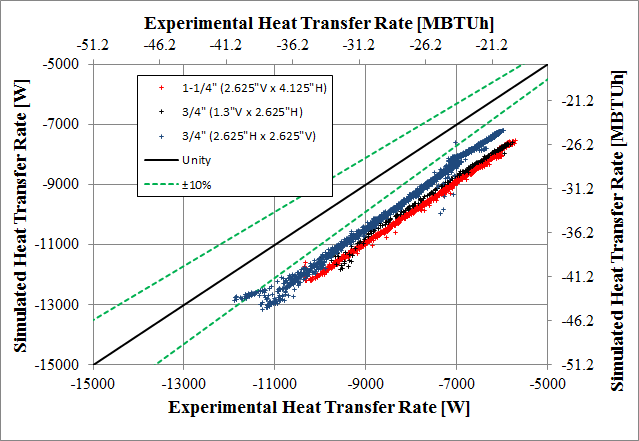
\includegraphics[width=0.8\textwidth]{HTChurchillPoolHE.png}
	\caption{Heat transfer rate comparison for the Churchill-Chu correlation vs.\ experimental pool heat extraction data}
	\label{fig:Correlation:Churchill:HTPoolHE}
\end{figure}

\subsection{Churchill-Chu Correlation Summary}
\label{Correlation:Churchill:Summary}

From the previous results, we can see that the correlation presented in this work better predicts the Nusselt number and heat transfer rates when compared to the \cite{ChurchillChu1975} convection correlation, which is what has been used up until this work. Table \ref{tab:Correlation:Churchill:SummaryTable} can be referenced to also to compare the current correlation against the \cite{ChurchillChu1975} convection correlation.

\begin{table}[h]
	\centering
	\caption{RMSE and MBE statistics for Nusselt number and heat transfer rate for the \cite{ChurchillChu1975} convection correlation}
	\label{tab:Correlation:Churchill:SummaryTable}
	\begin{tabular}{r | c c c c}
	\hline
	& \multicolumn{2}{c}{Nusselt Number} & \multicolumn{2}{c}{Heat Transfer Rate} \\
	& RMSE \% & MBE \% & RMSE \% & MBE \% \\
	\hline
	& \multicolumn{4}{c}{\textit{Mitchell/Churchill-Chu}} \\
	\hline\hline
	Pond HR & 27.1/41.9 & -6.5/-5.0 & 6.3/7.1 & -1.6/-1.2 \\
	\hline
	Quiescent HR & 6.9/92.6 & 0.0/90.2 & 2.5/15.4 & -0.1/15.2 \\
	\hline
	Pond HE & 12.2/44.9 & -1.8/38.4 & 5.0/11.8 & -0.8/10.3 \\
	\hline
	Quiescent HE & 9.1/99.6 & -4.5/97.4 & 4.1/21.6 & -2.0/21.0 \\
	\hline
	\end{tabular}
\end{table}

\section{Conclusions}
\label{sec:Correlation:Conclusions}

In this chapter, convection correlations have been developed for spiral-helical surface water heat exchangers. These correlations were developed from experimental data taken in a pond and pool in heat rejection and heat extraction modes of operation. The correlations have been shown to predict outside Nusselt number to within an RMSE value of 28\% for heat rejection cases, and within 13\% for heat extraction cases. When the correlations were implemented in a simulation, heat transfer rates were shown to be predicted to with 7\% RMSE for heat rejection cases, and within 5\% RMSE for heat extraction cases.

Revisited below is Equation \ref{eq:Correlation:PondHeatRej:CorrForm}, which is the general form of the correlation proposed in this chapter. Also shown below is Table \ref{tab:Correlation:Conclusion} where the correlation coefficients are summarized for the different SWHE operating conditions. Correlations labeled as quiescent are recommended for use in situations where the surface water body is shallow or the SWHE would by some other means be constrained. An example of this would be a situation where the pond level has dropped over the course of a hot summer to where the water level is very near the SWHE level. This would be expected to cause convective resistance to increase and system performance to decrease.

\begin{equation}
	\mbox{Nu}_{D,o} = a \cdot \left( b+ c \cdot \mbox{Ra}_{D,o}^{* \, d} \cdot \left(\frac{\Delta y}{D_o}\right)^{e} \cdot \left(\frac{\Delta x}{D_o}\right)^{f} \right)
	\tag{\ref{eq:Correlation:PondHeatRej:CorrForm} revisited}
\end{equation}

	\begin{table}[h]
		\centering
		\caption{Convection coefficient summary}
		\label{tab:Correlation:Conclusion}
		\begin{tabular}{r | c c c c c c}
			\hline
			Condition & a & b & c & d & e & f \\
			\hline\hline
			Pond HR & 1 & 5 & 0.0317 & 0.333 & 0.344 & 0.301 \\
			\hline
			Quiescent HR & 0.573 & 5 & 0.0317 & 0.333 & 0.344 & 0.301 \\
			\hline	
			Pond HE & 1 & 5.75 & 0.00971 & 0.333 & 0.929 & 0 \\
			\hline
			Quiescent HE & 0.87 & 5.75 & 0.00971 & 0.333 & 0.929 & 0 \\
			\hline		
		\end{tabular}
	\end{table}
	
Below, two tables are shown which give the range of applicability for each parameter in the outside convection correlation. Table \ref{tab:Correlation:PondHeatRej:RangeOfAppAgain} shows the range of applicability for the heat rejection mode of operation, while Table \ref{tab:Correlation:PoolHeatExtr:RangeOfAppAgain} shows the range of applicability for the heat extraction mode of operation.
	
	
	\begin{table}[h!]
		\centering
		\caption[Range of applicability for pond heat rejection correlation]{Range of applicability for heat rejection convection correlation}
		\label{tab:Correlation:PondHeatRej:RangeOfAppAgain}
		\begin{tabular}{r c c c l}
		0 & $\le$ &  $Ra_{D,o}^*$ & $\le$  & $6.0\cdot10^7$ \\
		1.3 in.\ (33 mm) & $\le$ & $\Delta y$ & $\le$ & 4.125 in.\ (105 mm) \\
		1.3 in.\ (33 mm) & $\le$ & $\Delta x$ & $\le$ & 4.125 in.\ (105 mm) \\
		1.05 in.\ (27 mm) & $\le$ &  $D_o$ &  $\le$ & 1.66 in.\ (42 mm) \\
		0.85 in.\ (22 mm) & $\le$ &  $D_i$ &  $\le$ & 1.36 in.\ (36 mm) \\
		\multicolumn{5}{c}{L = 500 ft.\ (153 m)} \\
		\end{tabular}
	\end{table}
	
	\begin{table}[h!]
		\centering
		\caption[Range of applicability for pool heat extraction correlation]{Range of applicability for heat extraction convection correlation}
		\label{tab:Correlation:PoolHeatExtr:RangeOfAppAgain}
		\begin{tabular}{r c c c l}
		$1.0\cdot10^6$ & $\le$ &  $Ra_{D,o}^*$ & $\le$  & $4.0\cdot10^7$ \\
		1.3 in.\ (33 mm) & $\le$ & $\Delta y$ & $\le$ & 2.625 in.\ (67 mm) \\
		2.625 in.\ (67 mm) & $\le$ & $\Delta x$ & $\le$ & 4.125 in.\ (105 mm) \\
		1.05 in.\ (27 mm) & $\le$ &  $D_o$ &  $\le$ & 1.66 in.\ (42 mm) \\
		0.85 in.\ (22 mm) & $\le$ &  $D_i$ &  $\le$ & 1.36 in.\ (36 mm) \\
		\multicolumn{5}{c}{L = 500 ft.\ (153 m)} \\
		\end{tabular}
	\end{table}
	
In the heat extraction mode of operation below $Ra_D^*=1\cdot10^6$, a constant Nusselt number of 5 should be applied. This is to account for the sensitivity of experimental data in this region due to the maximum density point of the surface water.